\documentclass[10pt,twocolumn]{article}
\usepackage[margin=0.72in]{geometry}
\usepackage[T1]{fontenc}
\usepackage{lmodern,booktabs,graphicx,amsmath,xcolor,url}
\usepackage[hidelinks]{hyperref}
\setlength{\columnsep}{0.24in}
\setlength{\parskip}{3pt}
\setlength{\parindent}{0pt}
\newcommand{\Acue}{A\textsubscript{cue}}
\newcommand{\pending}[1]{\textcolor{red!65!black}{[Pending: #1]}}
\title{Cue-Driven Keyframe Selection for Audio Description and Video QA\\\large PYRO-KD: Revision 1.5 experimental report draft}
\author{PYRO-KD team\\\small Agent Track; research project\\\small Human author names and individual contributions require team confirmation}
\date{Evidence snapshot: 23 November 2026}
\begin{document}
\maketitle
\begin{abstract}
Audio description requires selecting informative visual moments while fitting narration into dialogue gaps. PYRO-KD separates cue salience from placement feasibility, combining visual novelty, speech content, non-speech audio events, and voice-activity-derived gaps. We evaluate five selectors with two prompt priors and a planned two-model matrix, using REFRAMED as the primary benchmark. The authorized local portion uses a frozen Qwen2.5-VL model; paid API and human-label conditions are explicitly deferred. All 31 selector configurations have completed on 30 frozen test clips. Descriptive selector F1 is 0.311 for uniform, 0.389 for visual, 0.505 for audio-cue, 0.494 for fused selection, and 0.839 for the timestamp oracle. These are placement results before caption generation. A development pilot reveals material losses between requested moments, feasible inputs, valid captions, and individually speech-fitting narration. The formal local caption matrix completes 3,398 attempts with 3,108 valid captions and 3,024 individually speech-fitting renders. Audio-cue P0 reaches placement F1 0.521 versus 0.351 for V and 0.275 for U. All ten long-video QA conditions complete 360 valid answers; their thirteen video-clustered contrasts have Holm-adjusted $p=1.0$. EgoSchema heldout QA remains pending in this draft. The long-video audio conditions also have lower realized frame budgets than visual controls; they support constrained-budget diagnostics, not an equal-budget causal claim.
\end{abstract}

\section{Problem and experimental questions}
Inline audio description (AD) narrates visible events for blind and low-vision viewers without obscuring original dialogue. A salient event and a feasible narration slot need not occur at the same time. Audio cues can indicate events worth describing, but can also identify content already communicated by sound. Consequently, the sign of an audio-event contribution is an empirical question rather than an assumed benefit.

Revision 1.5 asks whether visual, audio, and fused selectors improve placement agreement over uniform sampling; whether events should trigger or suppress selection; whether guideline-based prompting improves descriptions; and whether selected frames and audio timelines improve downstream QA. A timestamp oracle measures reference-placement headroom, not a deployable method. This report separates evidence for those questions: temporal agreement, conditional reference-text similarity, actual synthesized-speech behavior, and QA correctness are different outcomes.

The experiments use frozen pretrained models with no fine-tuning. Human detector validation, blinded peer ratings, and calibrated rubric judging are necessary for claims about perceived description quality. Those measurements are not available here. Automated scores and agent inspection do not substitute for them.

\section{Method}
\subsection{Three audio streams and visual novelty}
Speech presence comes from Silero VAD; its intervals define candidate non-speech gaps. Speech content is transcribed with VAD-gated Whisper. Speech cues include semantic changes and visually referential phrases. Non-speech evidence uses AST AudioSet posteriors, CLAP embedding changes, and acoustic onset/loudness features. Speech and silence classes are excluded from the event interpretation. Optional speaker diarization is not available and is not claimed.

Visual features use cached OpenCLIP embeddings. Local novelty compares nearby embeddings; running-memory novelty considers already selected content. The audio-only proposal condition is \Acue{}, which uses speech and non-speech cues without visual features. A historical selector named A ranks gap quality; it is not silently substituted for \Acue{}.

\subsection{Selection, feasibility, and generation}
Each video requests $K=\max(1,\operatorname{round}(5T/60))$ moments for duration $T$ seconds. Core selectors are uniform U, visual V, audio-cue \Acue{}, fused AV, and reference timestamp oracle O. Candidate salience and gap feasibility are separate. The cue-driven variants identify candidate events, snap to eligible VAD gaps, and enforce two-second minimum separation. Four frames span two seconds around each selected placement timestamp. A finite candidate or gap supply can prevent realizing requested $K$; no arbitrary padding is applied.

The word budget is $\lfloor3\Delta t\rfloor$ for available gap duration $\Delta t$. P0 is the plain description prompt. P1 adds AD guidelines and three training-only exemplars. Both core prompts receive the same compact audio-timeline format. Generation uses temperature zero and flags outputs exceeding the word budget. Flagged and truncated outputs remain failures in coverage reports.

\section{Frozen evaluation protocol}
\subsection{Data and gates}
The primary evaluation is the existing 30-clip REFRAMED test subset, with a separate 10-clip development subset. Revision 1.5 explicitly permits reducing the originally larger test plan to 30 clips. Membership was not changed after seeing outcomes. P1 exemplars come from training only. Results refer to this defined subset, not every downloaded video.

All 5,031 distributed EgoSchema clips were verified to lack audio. Its heldout experiment therefore compares U, V-local, and V-memory as visual-only diagnostics on 490 videos, excluding 10 pilot videos. Audio-aware conclusions are not drawn from silent files.

The long-video benchmark is a frozen Video-MME subset: 12 videos, 36 questions, and approximately 7.7 hours of video. Source/license access and audio availability were checked before inference. There are ten conditions: U, V-local, flat \Acue{}, and flat AV without timelines; U, V-local, \Acue{}, and AV with flat selection and timelines; and hierarchical \Acue{} and AV with timelines. Global timelines contain at most 20 speech and 20 event entries, sampled independently of the question. No answer labels enter input preparation.

Cue2Narrate access and comparability remain unverified. No comparison against its published baselines is claimed. Human audio-event labels and peer judgments were deferred by the user. The detector gate therefore remains unvalidated, and event-class findings are explicitly exploratory.

\subsection{Models, development decisions, and controls}
The local core uses Qwen2.5-VL-7B snapshot \texttt{cc594898...}. The native-audio ablation uses Qwen2.5-Omni-7B snapshot \texttt{ae9e169...}. Full model paths and revisions are recorded in the frozen TOML and provenance files. Models run with bfloat16 and SDPA on A100 GPUs. Caption and EgoSchema frames use a 768-pixel maximum side; long-video QA uses 224 pixels following resource-only smokes with 612 and 1,012 frames. These different task resolutions are disclosed rather than treated as equivalent inputs.

Development tuning selected nonzero nuisance weights. For \Acue{}, non-speech-event, speech-cue, and gap-feasibility weights are each 0.5; for AV they are 0.5, 1.0, and 0.0. The chosen selector for audio-context ablation 5 is \Acue{}, based on development evidence. No test tuning is permitted.

The original development generation limit was 128 tokens. A separate 15-case development probe at 512 tokens rescued five responses, finishing in 128--139 tokens; ten continued looping to the limit. Formal generation is capped at 192 tokens. This decision covers the completed development responses while bounding persistent decoding failures. Original pilot outputs were preserved rather than relabeled as formal results.

\begin{table}[h]
\centering\small
\begin{tabular}{lrr}
\toprule Work & Conditions & Requests \\
\midrule REFRAMED local core & 10 & 3,398 \\
Paid core & 10 & Deferred \\
Native / no-context AD & 2 & 768 \\
EgoSchema heldout & 3 & 1,470 \\
Video-MME long & 10 & 360 \\
\bottomrule
\end{tabular}
\caption{Frozen inference scope. Timeline-present ablation outputs reuse the identical local core condition. Paid API authorization is \$0. Request counts do not imply successful outputs.}
\end{table}

\subsection{Metrics and statistical interpretation}
Temporal precision, recall, and F1 use one-to-one matching within $\pm2$ seconds. All selected test clips stay in the denominator, including clips with no feasible prepared moments or no valid predictions. Requested, selected, prepared, generated-valid, and rendered counts are reported separately.

BERTScore, sentence-embedding cosine, and OpenCLIP text similarity operate on temporally matched valid descriptions. They are conditional semantic proxies, not complete-coverage quality estimates. Actual Piper speech is rendered at 1.2$\times$ speed. We measure original-speech overlap, per-caption fit, and narration self-overlap separately. The latter is the sum of rendered durations minus their timeline union.

QA uses a strict standalone answer-letter parser and the complete frozen question denominator. Missing, invalid, and generation-error predictions count incorrect. Paired analyses use video/movie clusters, 10,000 bootstrap resamples, and Wilcoxon signed-rank tests. Declared contrast families receive Holm correction; 95\% bootstrap intervals are pointwise, not simultaneous. Newly specified core contrasts must not be represented as preregistered before any heldout output existed.

\section{Completed development evidence}
The development pilot executed all ten local selector--prompt cells. Across them, 1,110 requested moments became 1,008 selections, 804 prepared model inputs, 705 valid captions, and 688 individually speech-fitting renders. There were 84 word-budget failures and 15 token-limit failures. Among the 789 complete decodes with known word-budget status, 84 exceeded the cap (10.65\%). Truncated outputs have unknown complete-decode compliance and must not be classified as compliant.

\begin{figure}[h]
\centering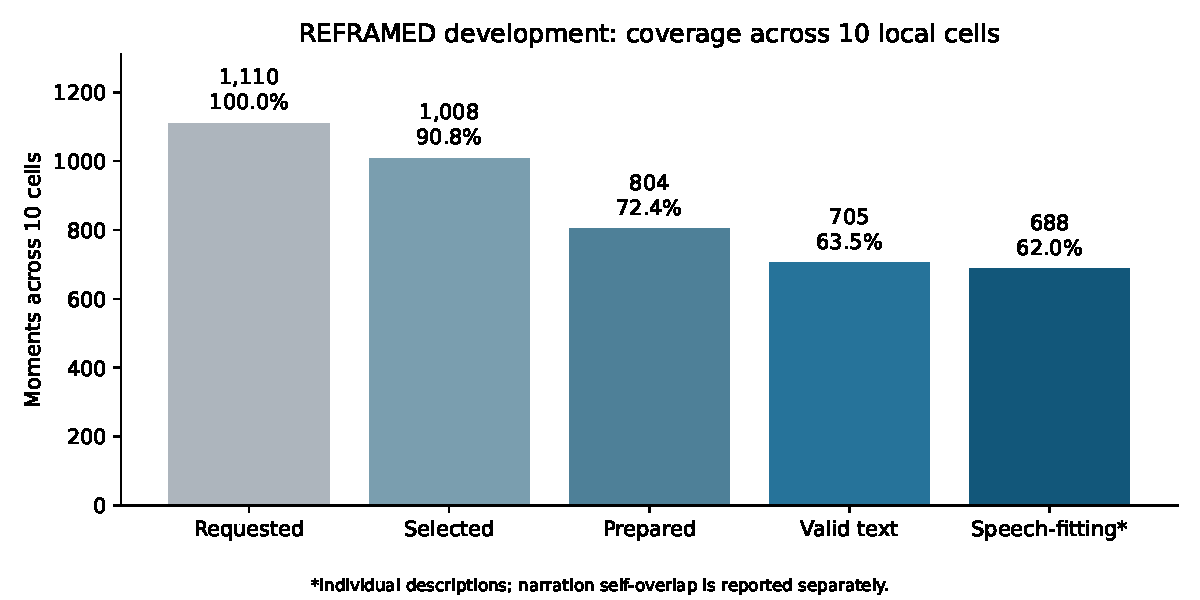
\includegraphics[width=\columnwidth]{../results/reframed-dev-coverage.pdf}
\caption{Development coverage across ten local cells. Each stage has a different denominator. Individual speech fit does not exclude overlap between AD captions.}
\end{figure}

\begin{table}[h]
\centering\small
\begin{tabular}{llrrr}
\toprule Selector & Prior & Valid/input & F1 & BERT \\
\midrule
U & P0 & 54/66 & 0.223 & 0.866 \\
U & P1 & 55/66 & 0.213 & 0.859 \\
V & P0 & 66/75 & 0.291 & 0.865 \\
V & P1 & 61/75 & 0.278 & 0.859 \\
A\_cue & P0 & 85/95 & 0.477 & 0.864 \\
A\_cue & P1 & 88/95 & 0.510 & 0.863 \\
AV & P0 & 83/95 & 0.462 & 0.866 \\
AV & P1 & 82/95 & 0.476 & 0.862 \\
O & P0 & 65/71 & 0.626 & 0.866 \\
O & P1 & 66/71 & 0.631 & 0.862 \\
\bottomrule
\end{tabular}

\caption{Development captions. F1 is placement F1 after failures; BERT is conditional BERTScore. These are development diagnostics, not heldout results.}
\end{table}

\subsection{Prompt audio-context diagnostic}
The development audio-context ablation holds the \Acue{}/P0 selected moments fixed at 95 and uses 30-second context windows. The no-audio-context condition produces 76 valid descriptions, the text-timeline condition 85, and native Omni 62. Corresponding placement F1 is 0.433, 0.477, and 0.408. Conditional BERTScore is 0.861, 0.864, and 0.867. All valid descriptions in this small ablation fit individually against original speech after rendering.

The native comparison changes both input modality and model architecture; it cannot identify an isolated effect of raw audio. Higher conditional similarity for a lower-coverage condition also does not establish better overall descriptions. The formal analysis below repeats the complete coverage accounting before interpreting score differences.

\subsection{Failure analysis}
Longer token ceilings do not repair all failures. Ten probe examples repeated phrases through 512 tokens; repeated bigrams appeared 39--111 times in individual outputs. Their text remains invalid and is excluded from semantic-quality summaries while remaining visible in coverage.

Two-second moment separation does not guarantee that complete narrations avoid each other. Development excess narration duration ranges from 65.9 seconds for U/P0 to 341.1 seconds for AV/P1 when aggregated over ten clips. Such overlap can occur even when each description individually avoids original speech. This exposes a scheduling limitation in the specified protocol. A future non-overlapping narration scheduler would be a separately declared method, not a silent correction to these runs.

The VAD-gated Whisper event baseline emits zero bracketed event tags on all ten development clips. This is an observed baseline limitation, not evidence that the clips contain no sounds. Human labels are needed to estimate event precision, missed sounds, or hallucinated tags; no such precision numbers are supplied here.

\section{Completed selector evidence}
All 31 frozen selector configurations cover all 30 test clips. Table~\ref{tab:selectors} shows the core selectors before caption preparation. The complete CSV and figure retain the speech-only/non-speech/both, trigger/suppress, event-source, event-time/snap, class-breakdown, and novelty-memory variants.

\begin{table}[h]
\centering\small
\begin{tabular}{lrrr}
\toprule Selector & Requested & Selected & F1 \\
\midrule
U & 388 & 388 & 0.311 \\
V & 388 & 388 & 0.389 \\
A\_cue & 388 & 384 & 0.505 \\
AV & 388 & 384 & 0.494 \\
O & 388 & 366 & 0.839 \\
\bottomrule
\end{tabular}

\caption{Heldout selector agreement, before caption generation. O is a reference timestamp upper bound. Scores are descriptive clip means.}\label{tab:selectors}
\end{table}

\section{Formal caption results and limitations}
\subsection{Core matrix and output availability}
All ten authorized local cells completed, with zero missing prepared IDs. Across them, 3,398 attempts yield 3,108 valid captions and 290 failures: 256 word-budget violations and 34 token-limit failures. Actual TTS renders all 3,108 valid captions; 3,024 fit individually against machine speech bounds. The complete 20-cell matrix retains ten API conditions as deferred (Table~\ref{tab:formal}). All 30 expected clips remain in each temporal denominator, including zero-output clips. Figure~\ref{fig:formalcoverage} separates the successive coverage losses.

\begin{table*}[t]
\centering\scriptsize
\begin{tabular}{lllrrrrrr}
\toprule Selector & Prior & Model & Valid/input & Failed & F1 & BERT & TTS fit/rendered & Zero-output clips \\
\midrule
U & P0 & Qwen & 255/283 & 28 & 0.275 & 0.863 & 246/255 & 3 \\
U & P0 & API & \multicolumn{6}{l}{Deferred: no paid authorization} \\
U & P1 & Qwen & 251/283 & 32 & 0.276 & 0.862 & 243/251 & 3 \\
U & P1 & API & \multicolumn{6}{l}{Deferred: no paid authorization} \\
V & P0 & Qwen & 266/305 & 39 & 0.351 & 0.866 & 258/266 & 4 \\
V & P0 & API & \multicolumn{6}{l}{Deferred: no paid authorization} \\
V & P1 & Qwen & 264/305 & 41 & 0.315 & 0.862 & 249/264 & 5 \\
V & P1 & API & \multicolumn{6}{l}{Deferred: no paid authorization} \\
A\_cue & P0 & Qwen & 372/384 & 12 & 0.521 & 0.867 & 370/372 & 0 \\
A\_cue & P0 & API & \multicolumn{6}{l}{Deferred: no paid authorization} \\
A\_cue & P1 & Qwen & 372/384 & 12 & 0.516 & 0.864 & 365/372 & 0 \\
A\_cue & P1 & API & \multicolumn{6}{l}{Deferred: no paid authorization} \\
AV & P0 & Qwen & 347/384 & 37 & 0.441 & 0.867 & 336/347 & 1 \\
AV & P0 & API & \multicolumn{6}{l}{Deferred: no paid authorization} \\
AV & P1 & Qwen & 341/384 & 43 & 0.441 & 0.865 & 331/341 & 1 \\
AV & P1 & API & \multicolumn{6}{l}{Deferred: no paid authorization} \\
O & P0 & Qwen & 322/343 & 21 & 0.669 & 0.867 & 315/322 & 3 \\
O & P0 & API & \multicolumn{6}{l}{Deferred: no paid authorization} \\
O & P1 & Qwen & 318/343 & 25 & 0.696 & 0.864 & 311/318 & 2 \\
O & P1 & API & \multicolumn{6}{l}{Deferred: no paid authorization} \\
\bottomrule
\end{tabular}

\caption{Formal REFRAMED core matrix: 30 frozen test clips per condition. F1 is clip-mean temporal placement of valid outputs; BERTScore is conditional on valid temporal matches. TTS fit is individual, not joint playback compatibility. O is an oracle upper bound. All paid cells remain visible as deferred.}\label{tab:formal}
\end{table*}

\begin{figure}[h]
\centering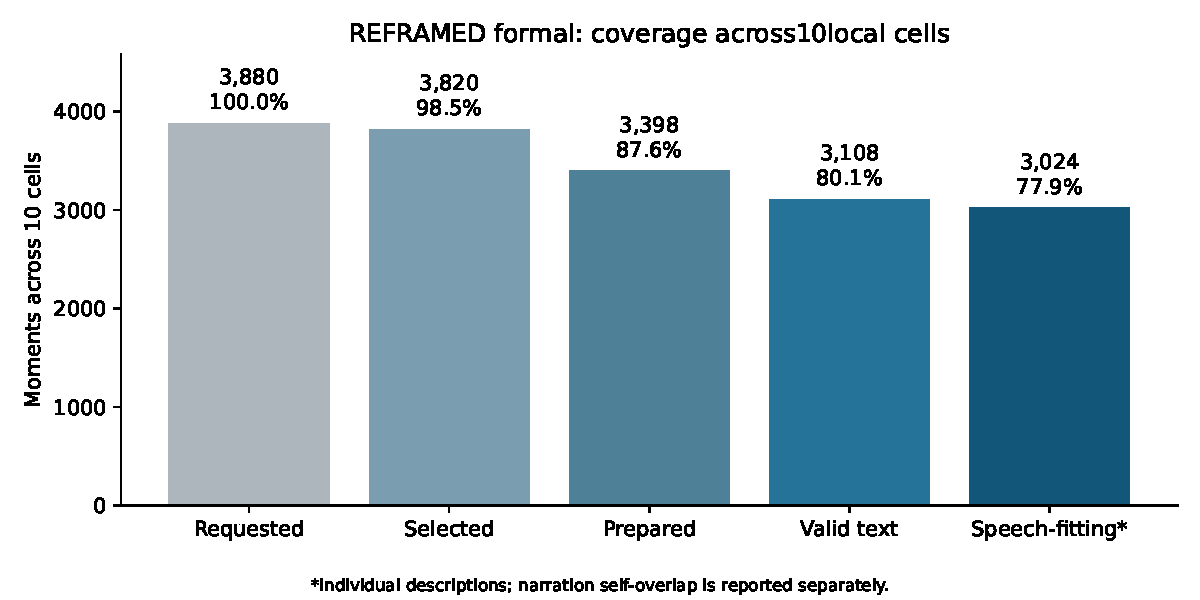
\includegraphics[width=\columnwidth]{../results/reframed-formal-core/coverage.pdf}
\caption{Formal local coverage across ten cells. Failures and feasibility losses are not dropped from the preceding stage's denominator.}\label{fig:formalcoverage}
\end{figure}

Audio-cue P0 obtains descriptive temporal F1 0.521 versus V at 0.351 and U at 0.275. The structural core family contains 17 contrasts over 10 movie clusters, declared after descriptive results were available rather than prospectively preregistered. Four contrasts have Holm-adjusted $p<0.05$: \Acue{}--V under P0; \Acue{}--U, \Acue{}--V, and AV--V under P1 (each adjusted $p=0.0332$). \Acue{}--U under P0 is $p=0.0508$, so it does not meet that cutoff. All five P1--P0 contrasts have adjusted $p=1.0$. These tests concern placement of valid outputs, not semantic or human quality. Pointwise bootstrap intervals are not familywise intervals, and separate families are not globally corrected.

\subsection{Formal audio-context ablation}
At the same 384 prepared \Acue{}/P0 moments, no-context Qwen produces 349 valid captions, timeline Qwen 372, and native Omni 326. Their temporal F1 values are 0.469, 0.521, and 0.465; individual speech-fit counts are 345/349, 370/372, and 324/326. The newly declared three-contrast movie-clustered family gives timeline minus no-context a mean F1 difference of 0.0519, pointwise 95\% interval [0.0107,0.1189], and Holm-adjusted $p=0.0410$. Native minus no-context has $p=0.7344$; native minus timeline has $p=0.0625$.

Crucially, timeline and no-context conditions use \emph{identical selected timestamps}. Their temporal-F1 difference therefore reflects which descriptions survive generation validity checks, not a change in selection or evidence of improved semantics. Native contrasts additionally change model architecture and modality. Conditional BERTScore is 0.860/0.867/0.871 for none/timeline/native, respectively, but cannot be promoted to a human preference claim.

\subsection{Measured gap use and targeted diagnostics}
Across all 30 clips, the machine VAD/Whisper-union gap denominator is 3,739.112 seconds per cell, including unused gaps and zero-output clips. Unique narration occupancy for \Acue{}/P0 is 54.56\%; its P1 condition occupies 61.46\%. These are measured speech-free occupancy fractions, not human-validated silence utilization. Individual fit also hides self-overlap: timeline \Acue{}/P0 has 729.971 excess narration seconds despite 370 individually fitting captions, and the ten local cells total 7,651.939 excess seconds. No revised scheduler was silently applied.

Targeted development frame inspection found a bounded grounding discrepancy: at \texttt{l5lLQICPOcnb\_A\_cue\_003}, the actual four images show men in a car, a plane releasing an object, the plane over a road, and a ground explosion. P0 describes standing men and a plane exploding, neither supported by those inputs. Separate traceable cases show a 0.325-second machine-speech collision for a word-compliant caption and a 0.429-second collision between two individually fitting narrations. These are agent-reviewed examples with source/frame/WAV hashes, not human labels or prevalence estimates.

Detector-defined audio associations identify 121 music onsets across 27 clips and 28 impulsive onsets across 12 clips, with descriptive reference-onset association lifts 1.317 and 1.258. Different weighting of reference starts and timeline duration prevents causal interpretation of those ratios. Only 9/548 reference starts fall in the predefined low-modeled-change subset; this is not a count of truly silent events. \Acue{} matches 0/9 of those starts, U 5/9, and V/AV 1/9 each. Human labels remain necessary for sound-event precision and missed-event claims. The 16 selector-ablation contrasts across 10 movies all have Holm-adjusted $p=1.0$; their family was also declared after descriptive results.

\subsection{Long-video QA and realized budget}
All ten long-video conditions complete 36/36 valid answers: 360 predictions with no missing, invalid, or generation-error rows. Table~\ref{tab:longqa} preserves the complete fixed denominator. The no-timeline controls use exactly the same frames as their flat timeline counterparts. Adding a timeline changes \Acue{} from 21/36 to 20/36 and AV from 20/36 to 18/36; the paired differences are $-0.0278$ (pointwise 95\% CI [$-0.1389$,0.0833]) and $-0.0556$ ([$-0.1667$,0.0556]). All thirteen declared video-clustered contrasts have Holm-adjusted $p=1.0$. These results provide no detected timeline or hierarchy benefit on this small subset; they do not prove absence of an effect.

\begin{table}[h]
\centering\scriptsize
\begin{tabular}{lrrl}
\toprule Condition & Correct/36 & Accuracy & 95\% CI \\
\midrule
U / none & 18 & 0.500 & [0.333,0.667] \\
V / none & 17 & 0.472 & [0.278,0.667] \\
U / timeline & 16 & 0.444 & [0.250,0.639] \\
V / timeline & 16 & 0.444 & [0.278,0.639] \\
A\_cue flat / timeline & 20 & 0.556 & [0.361,0.750] \\
A\_cue hier. / timeline & 20 & 0.556 & [0.361,0.750] \\
AV flat / timeline & 18 & 0.500 & [0.306,0.694] \\
AV hier. / timeline & 18 & 0.500 & [0.306,0.694] \\
A\_cue flat / none & 21 & 0.583 & [0.389,0.778] \\
AV flat / none & 20 & 0.556 & [0.361,0.750] \\
\bottomrule
\end{tabular}

\caption{Long Video-MME: 36 questions from 12 videos per condition, all valid. Intervals are pointwise video-bootstrap 95\% intervals. A/AV have fewer realized frames than U/V; cross-selector differences are constrained-budget diagnostics.}\label{tab:longqa}
\end{table}

Flat and hierarchical \Acue{} both score 20/36; their individual outcomes need not be identical, and their paired interval is [$-0.0833$,0.0833]. Flat and hierarchical AV both score 18/36 with a zero observed paired difference interval. The largest descriptive score, 21/36 for \Acue{} without a timeline, does not become a validated winner after the declared multiplicity correction. Per-video duration/frame-count results are retained in the exported length analysis rather than used to retune selection.

\pending{Insert the three490-question EgoSchema heldout results and their declared paired comparisons once all conditions finish.}

Long \Acue{} and AV cannot realize the same moment budget as U/V under the frozen safe-gap rule. Flat \Acue{} selects 1,497 of 2,314 requested moments (5,988 frames versus 9,256 for U). Other audio variants select 1,484--1,494 moments. A read-only capacity audit attributes most losses to eligible VAD-gap scarcity: video 604 requests 153 moments but has capacity 14, while VAD marks 97.4\% of its duration as speech. Greedy packing contributes only 15 further missing selections across the seven capacity-limited videos.

Therefore these audio-aware long-video results are constrained-budget diagnostics. Differences can reflect selection, audio context, and unequal realized frame count. They do not establish improved QA at equal realized visual budget. Arbitrary filling, relaxing the feasibility rule, or tuning on correctness would alter the research design. The present report retains the shortfall and identifies the unmet controlled comparison.

\subsection{Threats to validity}
The 30-clip REFRAMED subset and 12-video long subset are small. Clips from the same movie and questions from the same video are dependent, motivating clustered analysis. Bootstrap intervals do not cure limited representativeness. Reference placement is not unique: disagreement with a professional timestamp may still be usable AD, and agreement alone does not establish usefulness.

VAD and audio-event outputs are machine estimates. Without human detector labels, reported speech-free feasibility and event categories have unmeasured error. Text similarity can reward linguistic overlap without verifying visual grounding, and native audio can encourage descriptions of audible rather than visible content. These possible failure modes require systematic human or independently grounded analysis; they are not counted from intuition.

EgoSchema's silent distribution cannot support audio claims. Cue2Narrate access remains unavailable. Paid model conditions, rubric judging, 60 blinded peer comparisons, and detector labels are deferred. No fabricated annotations or proxy human ratings fill those rows. The available local experiments consequently do not complete every original proposal requirement.

\section{Reproducibility and current conclusion}
Frozen inference uses immutable worktrees and source/config/input fingerprints. The formal caption source is \texttt{09abb6c}; long audio QA uses \texttt{a7e0e1a}, and its visual controls use \texttt{1f5fb60}. Existing weights and feature caches are reused only after compatibility checks. Incremental changes and failures are recorded in the Agent Log; large data, weights, and raw outputs remain outside Git. The reproduction guide records commands, artifact roots, and stage prerequisites.

The completed evidence shows higher descriptive mean placement agreement for cue-driven selectors than uniform sampling on this frozen subset, while generation and narration introduce substantial additional failure modes. It does not yet establish better human-perceived AD or controlled-budget long-video QA. Formal caption results show a timeline-related improvement in valid-output availability under identical selected moments, without establishing semantic superiority. Long-video QA shows no contrast surviving its declared Holm family; matched-frame timeline controls do not improve descriptive accuracy. EgoSchema conclusions remain pending. All deferred human/API requirements and budget limitations remain explicit.

\begin{thebibliography}{9}\small
\bibitem{proposal} PYRO-KD team. \emph{Cue-Driven Keyframe Selection for Long-Video Audio Description \& QA: Revision 1.5}. Project proposal. Local snapshot: \texttt{docs/PROPOSAL\_REVISION\_1\_5.txt}.
\bibitem{repo} PYRO-KD repository and incremental experiment records. \url{https://github.com/Yvonne-Yu217/PYRO-KD}.
\bibitem{course} NYU CSCI-GA 2271. Project requirements, Agent Track. \url{https://www.sainingxie.com/cv-fall2026/project/}. Accessed 23 November 2026.
\end{thebibliography}

\clearpage
\appendix
\section{Agent Log appendix}
This appendix summarizes agent contributions and failures. The full chronological English record is \texttt{docs/AGENT\_LOG.md}; the source and artifacts in that log remain authoritative. This draft does not attribute unverified work to human team members.

\subsection{Division of work and tools}
The user specified the research objective, resumption constraints, no paid API authorization, and deferral of human labels. Human authorship, implementation contributions, and manual diagnoses prior to this run must be confirmed by the team before submission. Agents audited the repository and scheduler, integrated readiness fixes in isolated worktrees, inspected dataset gates, prepared compatible cache adapters, wrote and ran regression tests, scheduled inference, assembled metric reports, and drafted this document.

Tools included shell/Python, Git and GitHub, Slurm, Singularity read-only environments, PyTorch/Transformers, cached pretrained speech/audio/vision models, pytest, and CPU plotting/TTS utilities. Parallel agents prepared inputs, audited long-video budget capacity, implemented statistical exports, and assembled report artifacts. Workers coordinate output ownership and GPU locks. They do not modify code under live jobs.

\subsection{Where agents and integrations failed}
\textbf{Stale output reuse.} The earlier experiment runner could reuse outputs after changes to configuration. The repair binds source files, normalized configuration, split membership, and exemplar identity. Legacy outputs without compatible identity are rejected rather than silently adopted. Regression tests exercise changed inputs and safe reuse.

\textbf{Coverage hidden by existing outputs.} Missing videos could disappear from evaluation denominators. Evaluation now reports expected membership, missing and unexpected IDs, and zero-output examples. Semantic scores remain conditional and are labeled accordingly.

\textbf{Ledger and interrupted-output handling.} Relative API ledgers could resolve inconsistently. Ledgers now resolve to absolute paths. Truncated JSONL recovery accepts only an unterminated final fragment, backs up the original, and repairs atomically; corruption inside the file fails. No paid request was required to validate these paths.

\textbf{Cross-branch interface assumptions.} PR and HPC audio caches used different schemas. Recomputing all features would have wasted resources. A validated adapter reuses speech/event/onset caches and preserves their provenance. Prompt/timeline and QA interface mismatches were exposed by initial failing tests, then corrected before scaling.

\textbf{Native-model invocation.} The installed Omni wrapper did not support the assumed generation route. The backend disables talker generation and calls the thinker directly; a real native-audio smoke verified this route before the ablation.

\textbf{Metric denominator mistake.} Word-budget violations were flagged as errors, then omitted by valid-only compliance aggregation, making the reported over-budget rate appear zero. The corrected metric includes complete flagged decodes in the known denominator, keeps truncated/backend failures unknown, and exposes missing outputs separately. Development recalculation recovered 84 violations among 789 known decodes. Temporal/semantic valid-output rules were not silently redefined.

\textbf{Cache-return validation mistake.} The first EgoSchema CPU driver validated a pre-publication return dictionary lacking an embedding path, falsely failing after writing usable caches. The repair reloads published metadata, verifies arrays/frame paths/hashes, and reuses compatible outputs. False-negative logs remain retained; a failed Slurm exit alone does not establish that extraction must be repeated.

\textbf{Wrong TTS cache path.} A formal CPU overlap watcher pointed at the development cache, failing after rendering the first cell. The external watcher was corrected to the formal test cache and reused rendered audio. Inference source remained frozen and the failed log was retained.

\textbf{Budget interpretation.} A nominal fixed-$K$ long-video configuration did not imply equal realized frames. Capacity auditing exposed gap-constrained shortfalls. The interpretation was narrowed to a diagnostic instead of padding inputs, inventing evidence, or claiming the original controlled comparison had passed.

\textbf{Missing timeline controls.} An audit of the initial long-QA queue found missing timeline-absent controls for audio-only and fused selection. The queue was expanded from eight to ten conditions before correctness scoring, adding 72 requests with exactly the same frame lists, times, questions, and options as their timeline counterparts. The contrast family was expanded from nine to thirteen before labels were opened. This repairs experimental completeness; it is not outcome-driven tuning.

\subsection{Verification evidence and remaining work}
The exact formal source passed 817 tests, with three skips and 5,974 subtests, recorded in \path{/scratch/yy5919/pyro-formal-source-full-tests.log}. Focused regressions additionally exercised budget denominators, JSONL recovery, coverage, identity guards, QA error handling, and cache validation. Development GPU smokes used real data, followed by the complete local pilot and actual 1.2$\times$ TTS evaluation. Long-QA resource tests validated 612- and 1,012-frame inference without inspecting correctness.

Verification also includes raw prediction counts, unique IDs, source hashes, frozen split checks, expected-video denominators, and separate accounting of zero-feasible and failed examples. GPU telemetry and Slurm job records establish execution, but are not substitutes for output validation. Test counts alone likewise do not establish scientific validity.

Human detector labels, blinded peer judgments, paid-model comparisons, and rubric calibration remain outstanding by explicit authorization limits. Human contribution attribution and a team code walkthrough remain submission responsibilities. The team should inspect the final tables, explain the fixes above, and replace every pending result slot only with verified artifacts.
\end{document}
